% \documentclass[compress]{beamer} % full
\documentclass[handout,compress]{beamer} % no animations

\usepackage{etex} % necessary for pgfplots

\usetheme{AGH}

\graphicspath{{figures/}}
\hypersetup{colorlinks, pdfstartview=FitH, bookmarksopen, pdfpagemode=UseNone, pdfpagemode=UseOutlines, linkcolor=black, citecolor=black, filecolor=black, urlcolor=black, pdfauthor={Piotr Cholda}}

% Not all of the following packages are necessary, but the teacher uses many of them :)
% \usepackage{algorithm}
% \usepackage{algpseudocode}
% \usepackage{amsmath,amsfonts}
% \usepackage{amssymb}
% \usepackage{array,supertabular}
\usepackage{bibentry}
% \usepackage{bm}
\usepackage{booktabs}
% \usepackage{cases}
\usepackage{cite}
\usepackage{color}
\definecolor{gold}{HTML}{E6B800}
\definecolor{lightgreen}{HTML}{99CC00}
\definecolor{blue}{HTML}{4D94DB}
\usepackage{colortbl}
\usepackage{comment}
% \usepackage{dsfont}
\usepackage{enumerate}
\usepackage{exscale,relsize}
\usepackage{floatflt}
\usepackage[OT4]{fontenc}
\usepackage{graphicx}
\usepackage[latin2]{inputenc}
% \usepackage{longtable}
% \usepackage{marvosym}
% \usepackage{multirow}
\usepackage{nicefrac}
\usepackage{paralist}
\usepackage{rotating}
\usepackage[tight,footnotesize]{subfigure}
\usepackage{tabularx}
\usepackage{tabulary}
\usepackage{tikz}
\usetikzlibrary{arrows}
\usetikzlibrary{automata}
\usetikzlibrary{backgrounds}
\usetikzlibrary{calc}
\usetikzlibrary{decorations.pathreplacing}
\usetikzlibrary{decorations.pathmorphing}
\usetikzlibrary{fit}
\usetikzlibrary{matrix}
\usetikzlibrary{mindmap}
\usetikzlibrary{patterns}
\usetikzlibrary{petri}
\usetikzlibrary{positioning}
\usetikzlibrary{plothandlers}
\usetikzlibrary{plotmarks}
\usetikzlibrary{shadings}
\usetikzlibrary{shadows}
\usetikzlibrary{shapes}
\usetikzlibrary{shapes.gates.logic.US}
\usetikzlibrary{topaths}
\usetikzlibrary{trees}
\usepackage{pgfplots} % needs \usepackage{etex} just after \documentclass
\pgfplotsset{tick scale binop=\times}

\usepackage{trfsigns}
\usepackage{url}
\usepackage{wasysym}
\usepackage{wrapfig}

\setbeamertemplate{footline}[text line]{
    \leavevmode
    \hbox{
        \begin{beamercolorbox}[wd=\paperwidth,ht=0.01ex,dp=0ex,leftskip=0.25cm,rightskip=0cm plus1fil]{title in head/foot}
            \usebeamerfont{title in head/foot}\logosinfootline
        \end{beamercolorbox}
    }
}

\setbeamertemplate{frametitle continuation}[from second][\insertcontinuationtext]

\setbeamercovered{dynamic}
\definecolor{lightgreen}{RGB}{218,238,225}
\setbeamercolor{rafi}{fg=lightgreen,bg=}

\newenvironment{changemargin}[2]{%
    \begin{list}{}{%
        \setlength{\topsep}{0pt}%
        \setlength{\leftmargin}{#1}%
        \setlength{\rightmargin}{#2}%
        \setlength{\listparindent}{\parindent}%
        \setlength{\itemindent}{\parindent}%
        \setlength{\parsep}{\parskip}%
    }%
    \item[]}
{\end{list}}

% \bstctlcite
\makeatletter
    \def\bstctlcite#1{\@bsphack
    \@for\@citeb:=#1\do{%
    \edef\@citeb{\expandafter\@firstofone\@citeb}%
    \if@filesw\immediate\write\@auxout{\string\citation{\@citeb}}\fi}%
    \@esphack}
\makeatother

\newtheorem{remark}{Remark}[theorem]

\abovedisplayshortskip=0pt

\DeclareMathOperator*{\argmin}{arg\,min}

\DeclareMathOperator*{\erf}{erf}

\DeclareMathOperator*{\rank}{rank}

\DeclareMathOperator*{\Dom}{Dom}

\DeclareMathOperator*{\opt}{opt}

\DeclareMathOperator*{\conv}{conv}

\DeclareMathOperator*{\diff}{\!\text{d}}

\DeclareMathOperator*{\mean}{\text{E}}

\DeclareMathOperator*{\logistic}{\text{logistic}}

\newcommand{\eqdef}{%
      \ensuremath{%
          \stackrel{\text{def}}{=}%
      }%
  }

%%%%%%%%%%%%%%%%%%%%%%%%%%%%%%%%%%%%%%%%%%%%%%%%%%%%%%%%%%%%%%%%%%%%%%%%%%%%%%%%%%%%%%%%%%%%%%%%%%%
%%%%%%%%%%%%%%%%%%%%%%%%%%%%%%%%%%%%%%%%%%%%%%%%%%%%%%%%%%%%%%%%%%%%%%%%%%%%%%%%%%%%%%%%%%%%%%%%%%%
%%%%%%%%%%%%%%%%%%%%%%%%%%%%%%%%%%%%%%%%%%%%%%%%%%%%%%%%%%%%%%%%%%%%%%%%%%%%%%%%%%%%%%%%%%%%%%%%%%%
%%%%%%%%%%%%%%%%%%%%%%%%%%%%%%%%%%%%%%%%%%%%%%%%%%%%%%%%%%%%%%%%%%%%%%%%%%%%%%%%%%%%%%%%%%%%%%%%%%%
%%%%%%%%%%%%%%%%%%%%%%%%%%%%%%%%%%%%%%%%%%%%%%%%%%%%%%%%%%%%%%%%%%%%%%%%%%%%%%%%%%%%%%%%%%%%%%%%%%%
\title%<<<<<<<<<<<<<<<<<<<<<<<<<<<<<<<<<<<<<<<<<<<<<<<<<<<<<<<<<<<<<<<<<
{Seminar in \emph{Course Name}}
\subtitle{Topic of the Seminar Presentation} % Change, please!
\author[]{Presenters} % Change, please!
\institute[KT AGH]{Department of Telecommunications}%
\date{Date} % Change, please!
%%%%%%%%%%%%%%%%%%%%%%%%%%%%%%%%%%%%%%%%%%%%%%%%%%%%%%%%%%%%%%%%%%%%%%%%%%%%%%%%%%%%%%%%%%%%%%%%%%%
%%%%%%%%%%%%%%%%%%%%%%%%%%%%%%%%%%%%%%%%%%%%%%%%%%%%%%%%%%%%%%%%%%%%%%%%%%%%%%%%%%%%%%%%%%%%%%%%%%%
%%%%%%%%%%%%%%%%%%%%%%%%%%%%%%%%%%%%%%%%%%%%%%%%%%%%%%%%%%%%%%%%%%%%%%%%%%%%%%%%%%%%%%%%%%%%%%%%%%%
%%%%%%%%%%%%%%%%%%%%%%%%%%%%%%%%%%%%%%%%%%%%%%%%%%%%%%%%%%%%%%%%%%%%%%%%%%%%%%%%%%%%%%%%%%%%%%%%%%%
%%%%%%%%%%%%%%%%%%%%%%%%%%%%%%%%%%%%%%%%%%%%%%%%%%%%%%%%%%%%%%%%%%%%%%%%%%%%%%%%%%%%%%%%%%%%%%%%%%%

\begin{document}

\begin{frame}
    \titlepage
    \nobibliography* % Necessary if literature is given
\end{frame}

\setbeamertemplate{background}{
\includegraphics[width=\paperwidth,height=\paperheight]{./files/tlo}}

\renewcommand{\logosinfootline}{\raisebox{0.12cm}{\begin{beamercolorbox}{rafi}{Seminar \quad Topic (change, please!) \hfill \insertframenumber/\inserttotalframenumber}\end{beamercolorbox}}}

\begin{frame}[allowframebreaks]
    \frametitle{Outline}
    \tableofcontents
\end{frame}


%%%%%%%%%%%%%%%%%%%%%%%%%%%%%%%%%%%%%%%%%%%%%%%%%%%%%%%%%%%%%%%%%%%%%%%%%%%%%%%%%%%%%%%%%%%%%%%%%%%
%%%%%%%%%%%%%%%%%%%%%%%%%%%%%%%%%%%%%%%%%%%%%%%%%%%%%%%%%%%%%%%%%%%%%%%%%%%%%%%%%%%%%%%%%%%%%%%%%%%
%%%%%%%%%%%%%%%%%%%%%%%%%%%%%%%%%%%%%%%%%%%%%%%%%%%%%%%%%%%%%%%%%%%%%%%%%%%%%%%%%%%%%%%%%%%%%%%%%%%
%%%%%%%%%%%%%%%%%%%%%%%%%%%%%%%%%%%%%%%%%%%%%%%%%%%%%%%%%%%%%%%%%%%%%%%%%%%%%%%%%%%%%%%%%%%%%%%%%%%
%%%%%%%%%%%%%%%%%%%%%%%%%%%%%%%%%%%%%%%%%%%%%%%%%%%%%%%%%%%%%%%%%%%%%%%%%%%%%%%%%%%%%%%%%%%%%%%%%%%

\section{Topic of the Presentation} % Change, please!

\begin{frame}
	\frametitle{Introduction}
	
	\begin{center}
		\Huge {What is word embedding?}
	\end{center}
\end{frame}



\begin{frame}
	\frametitle{Introduction}
	
	
		\huge {What a \textbf{lovely} day.}
		 \newline
		\huge{What a \textbf{nice} day.}

\end{frame}

\begin{frame}
	\frametitle{Introduction}
	
	
		\huge {What = [1, 0, 0, 0, 0]}
		 \newline
		\huge{a = [0, 1, 0, 0, 0]}
		\newline
		\huge{lovely = [0, 0, 1, 0, 0]}
		\newline
		\huge{nice = [0, 0, 0, 1, 0]}
		\newline
		\huge{day = [0, 0, 0, 0, 1]}

\end{frame}

\begin{frame}
	\frametitle{Word Embedding}

	\begin{figure}
		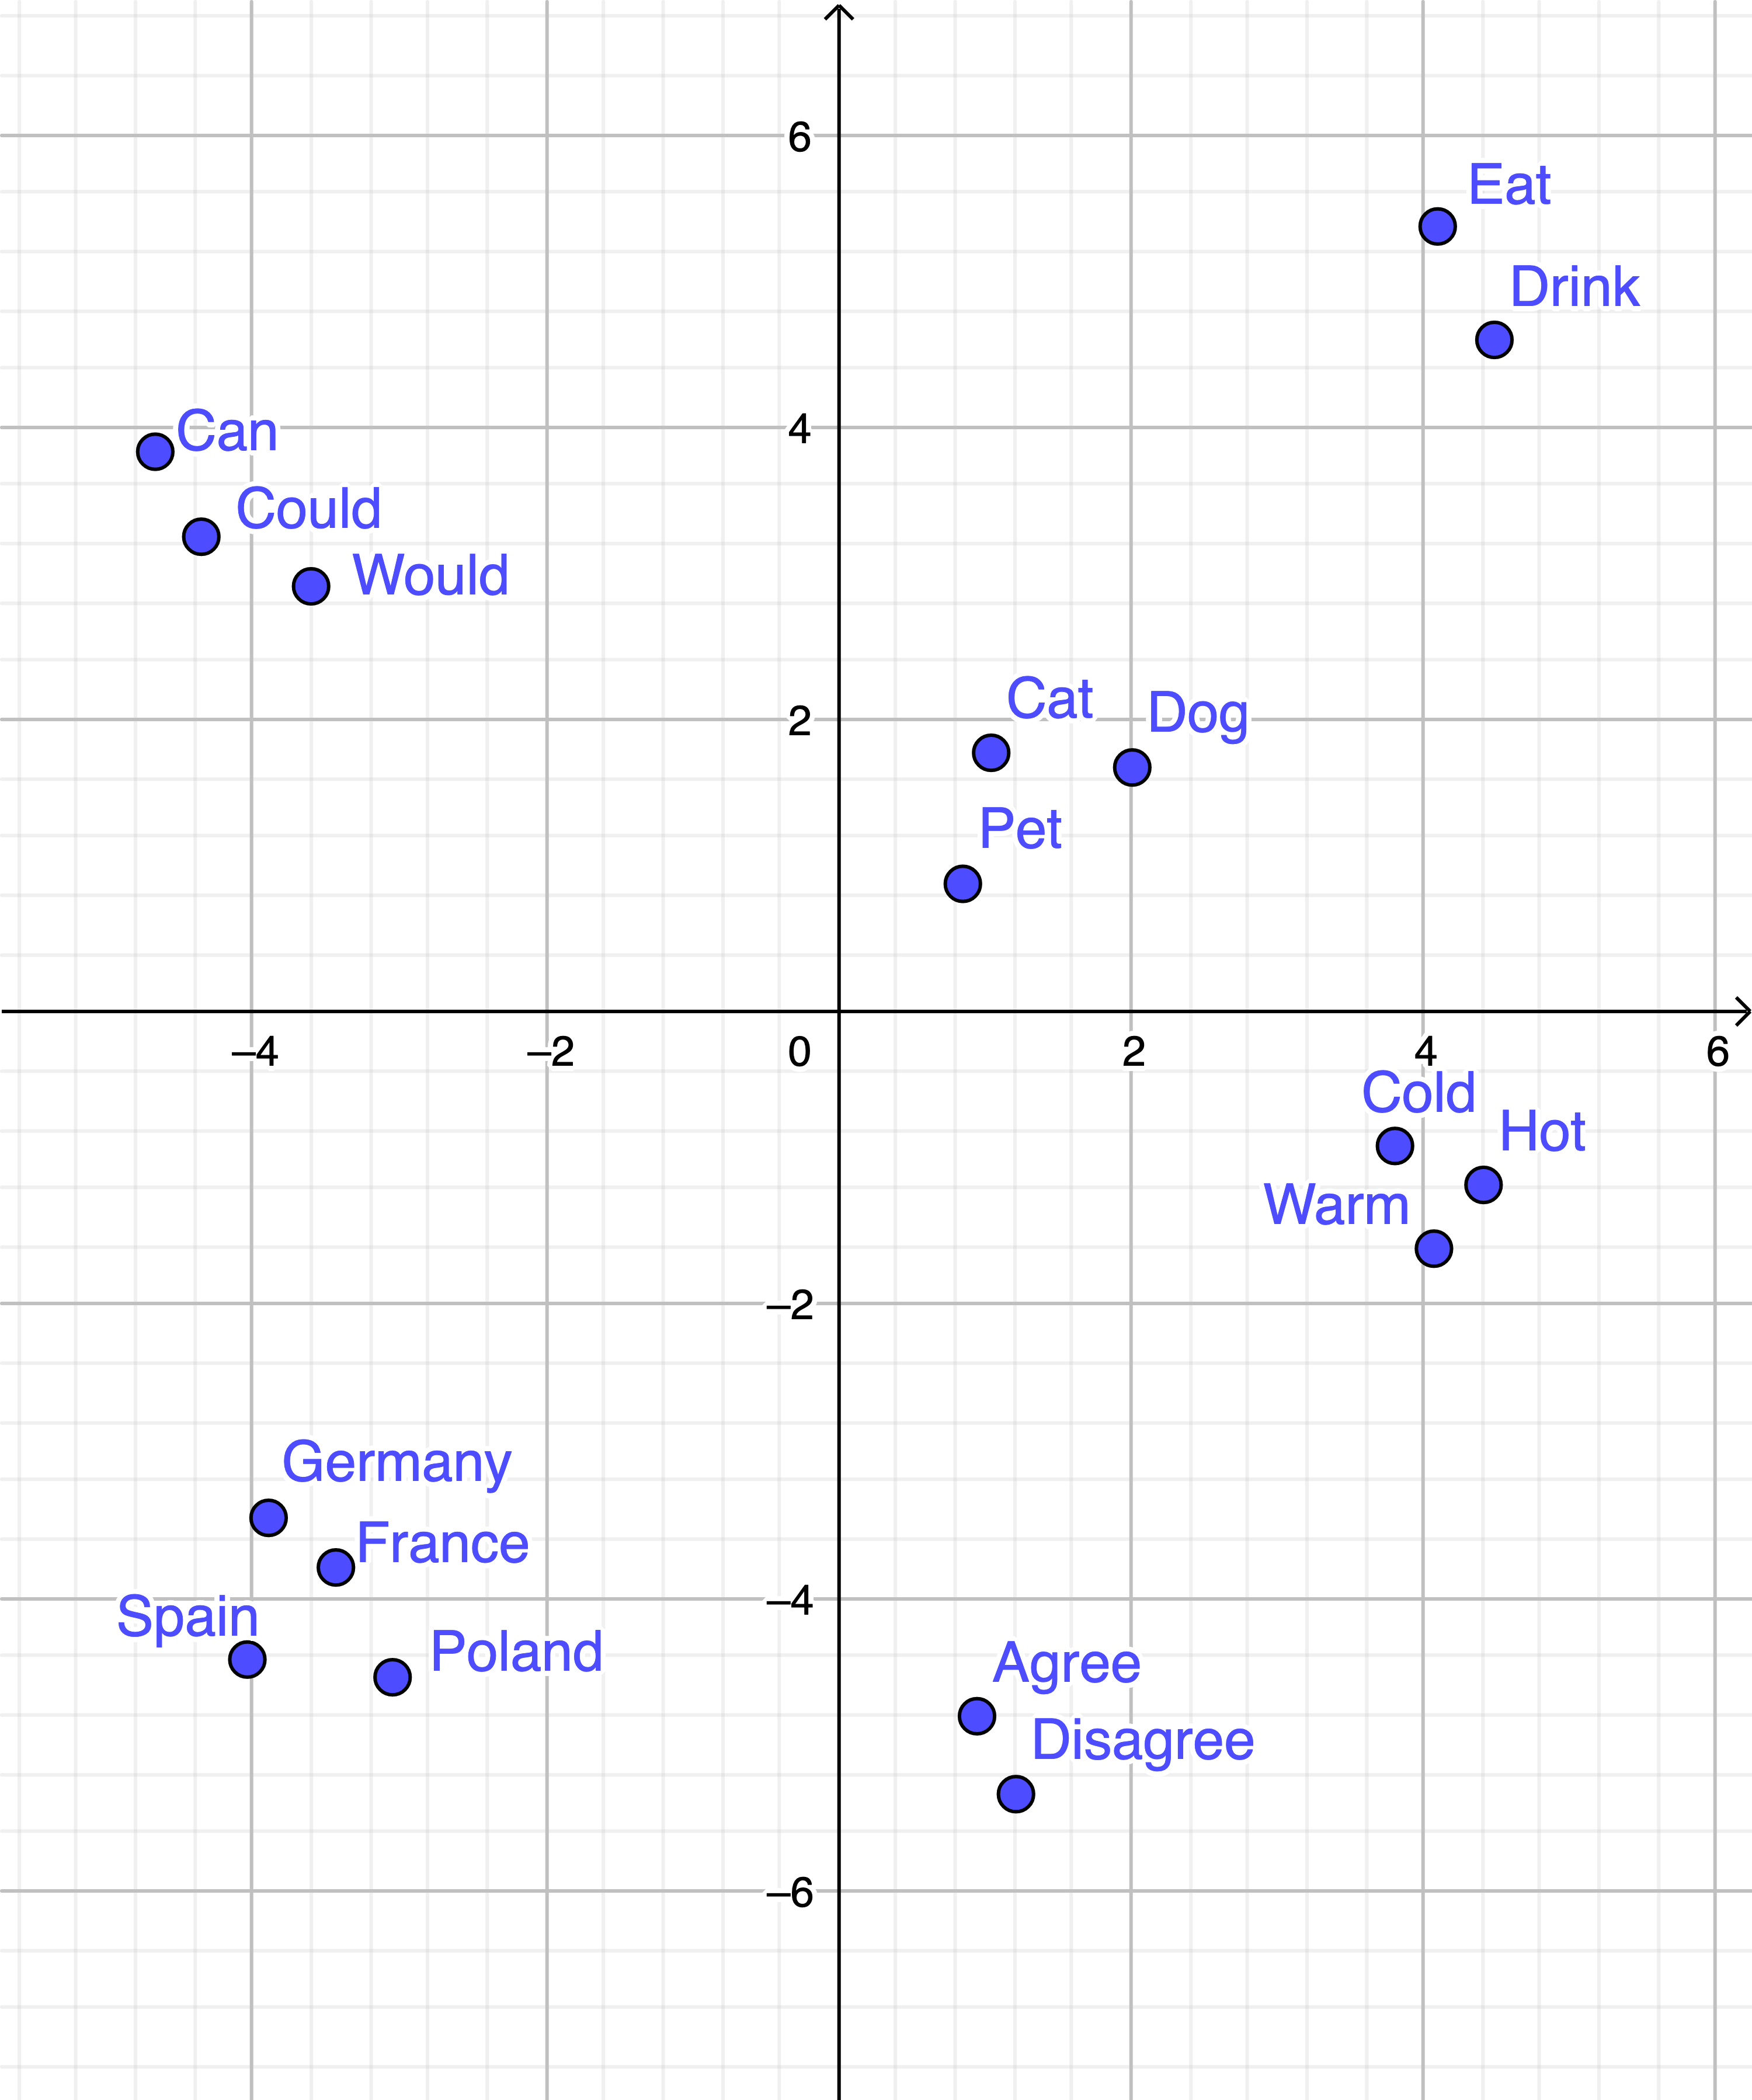
\includegraphics[width=4cm]{./figures/Groups}

	\end{figure}
		\begin{center}
		{Caption of the figure}
		\end{center}
	\vspace{-0.5cm}



\end{frame}

\begin{frame}
	\frametitle{Word Embedding}

	\begin{figure}
		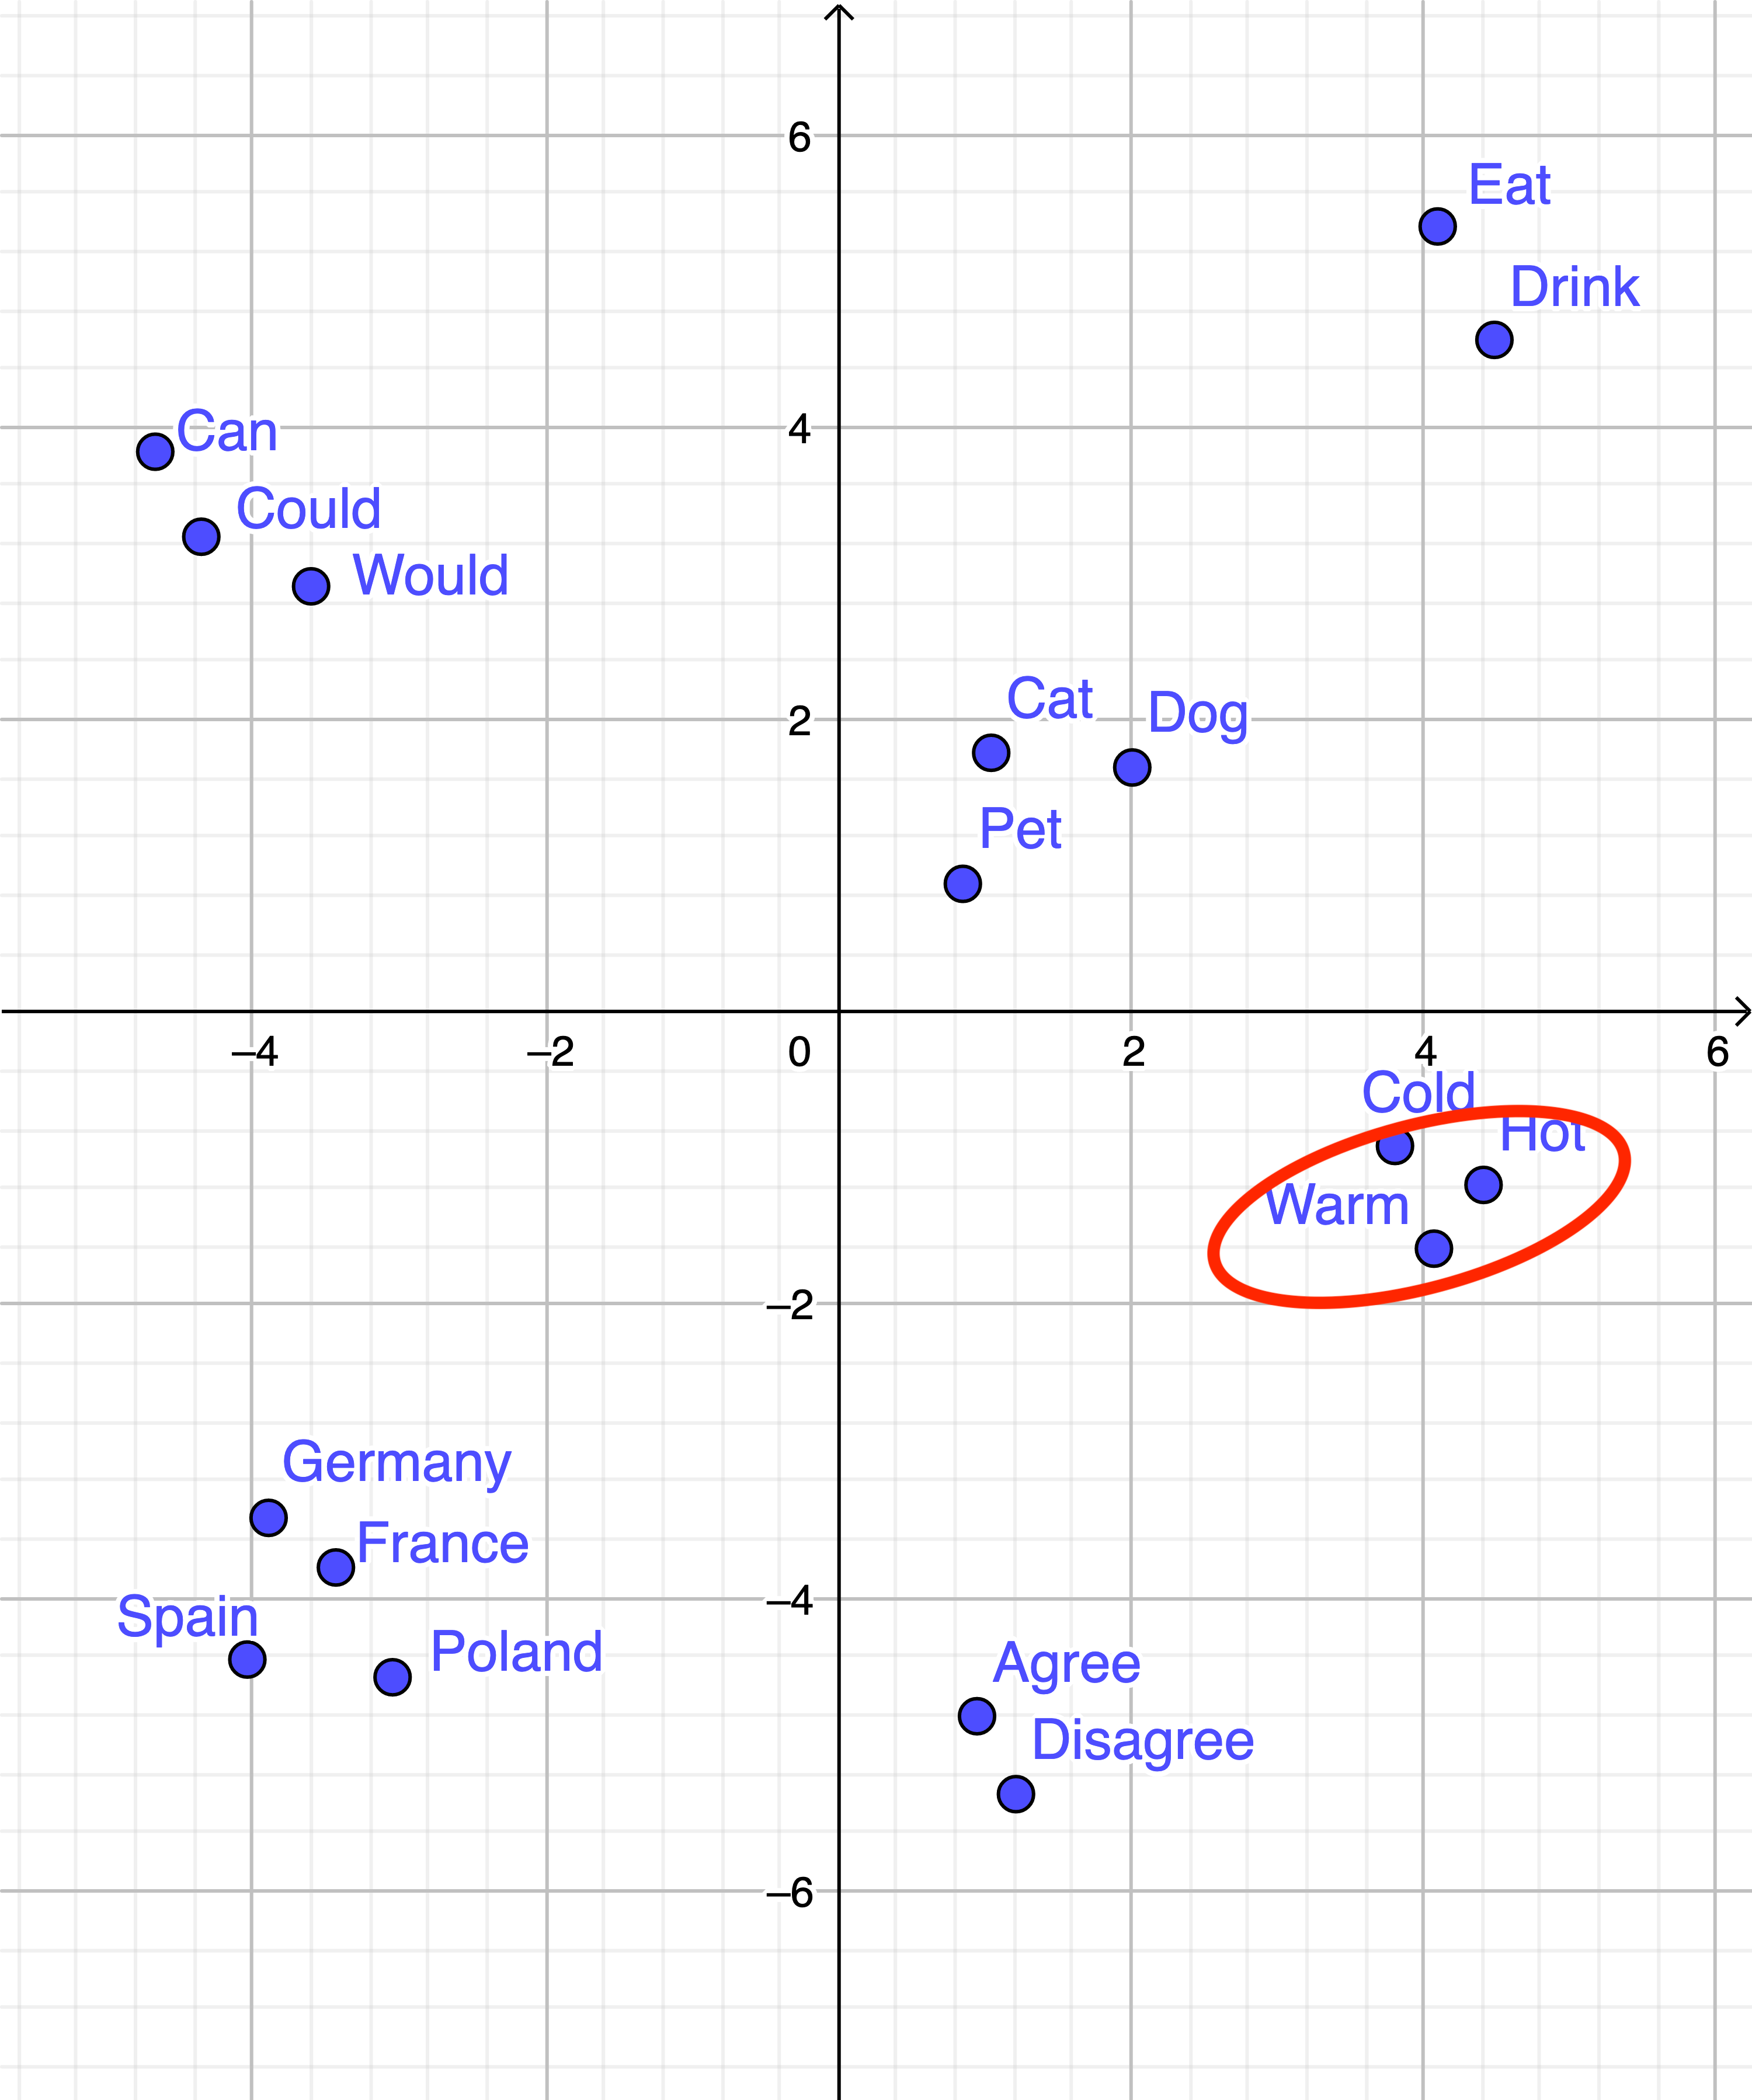
\includegraphics[width=4cm]{./figures/Group_synonym}

	\end{figure}
		\begin{center}
		{Words are synonyms}
		\end{center}
	\vspace{-0.5cm}

\end{frame}

\begin{frame}
	\frametitle{Word Embedding}

	\begin{figure}
		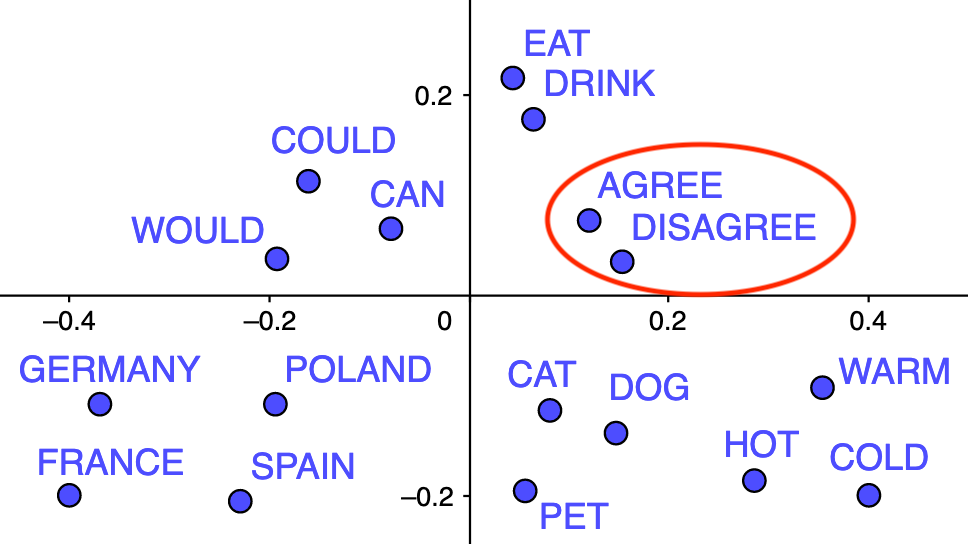
\includegraphics[width=4cm]{./figures/Group_antonyms}

	\end{figure}
		\begin{center}
		{Words are antonyms}
		\end{center}
	\vspace{-0.5cm}

\end{frame}

\begin{frame}
	\frametitle{Word Embedding}
		\framesubtitle{Slide with a Figure from a File}

	\begin{figure}
		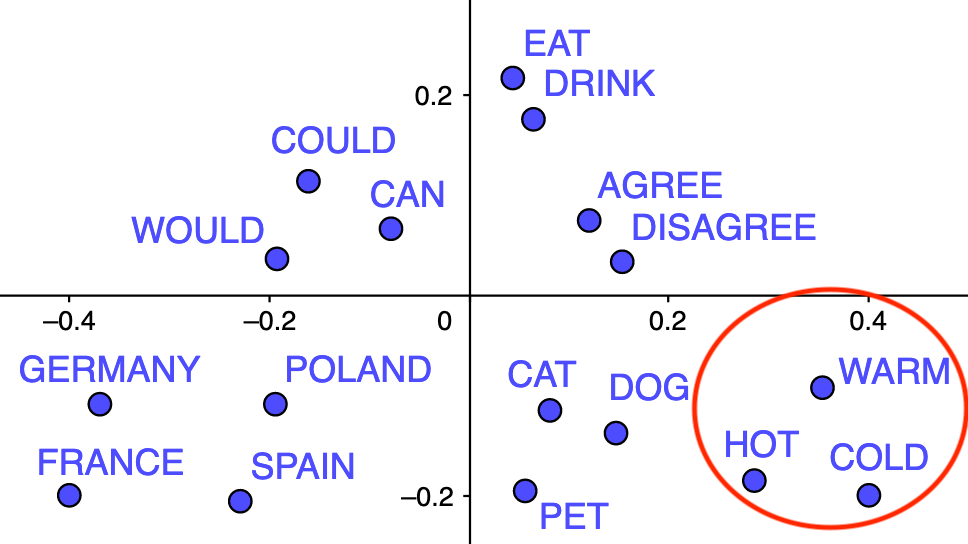
\includegraphics[width=4cm]{./figures/Group_scale}

	\end{figure}
		\begin{center}
		{Words are value on a scale}
		\end{center}
	\vspace{-0.5cm}

\end{frame}

\begin{frame}
	\frametitle{Word Embedding}

	\begin{figure}
		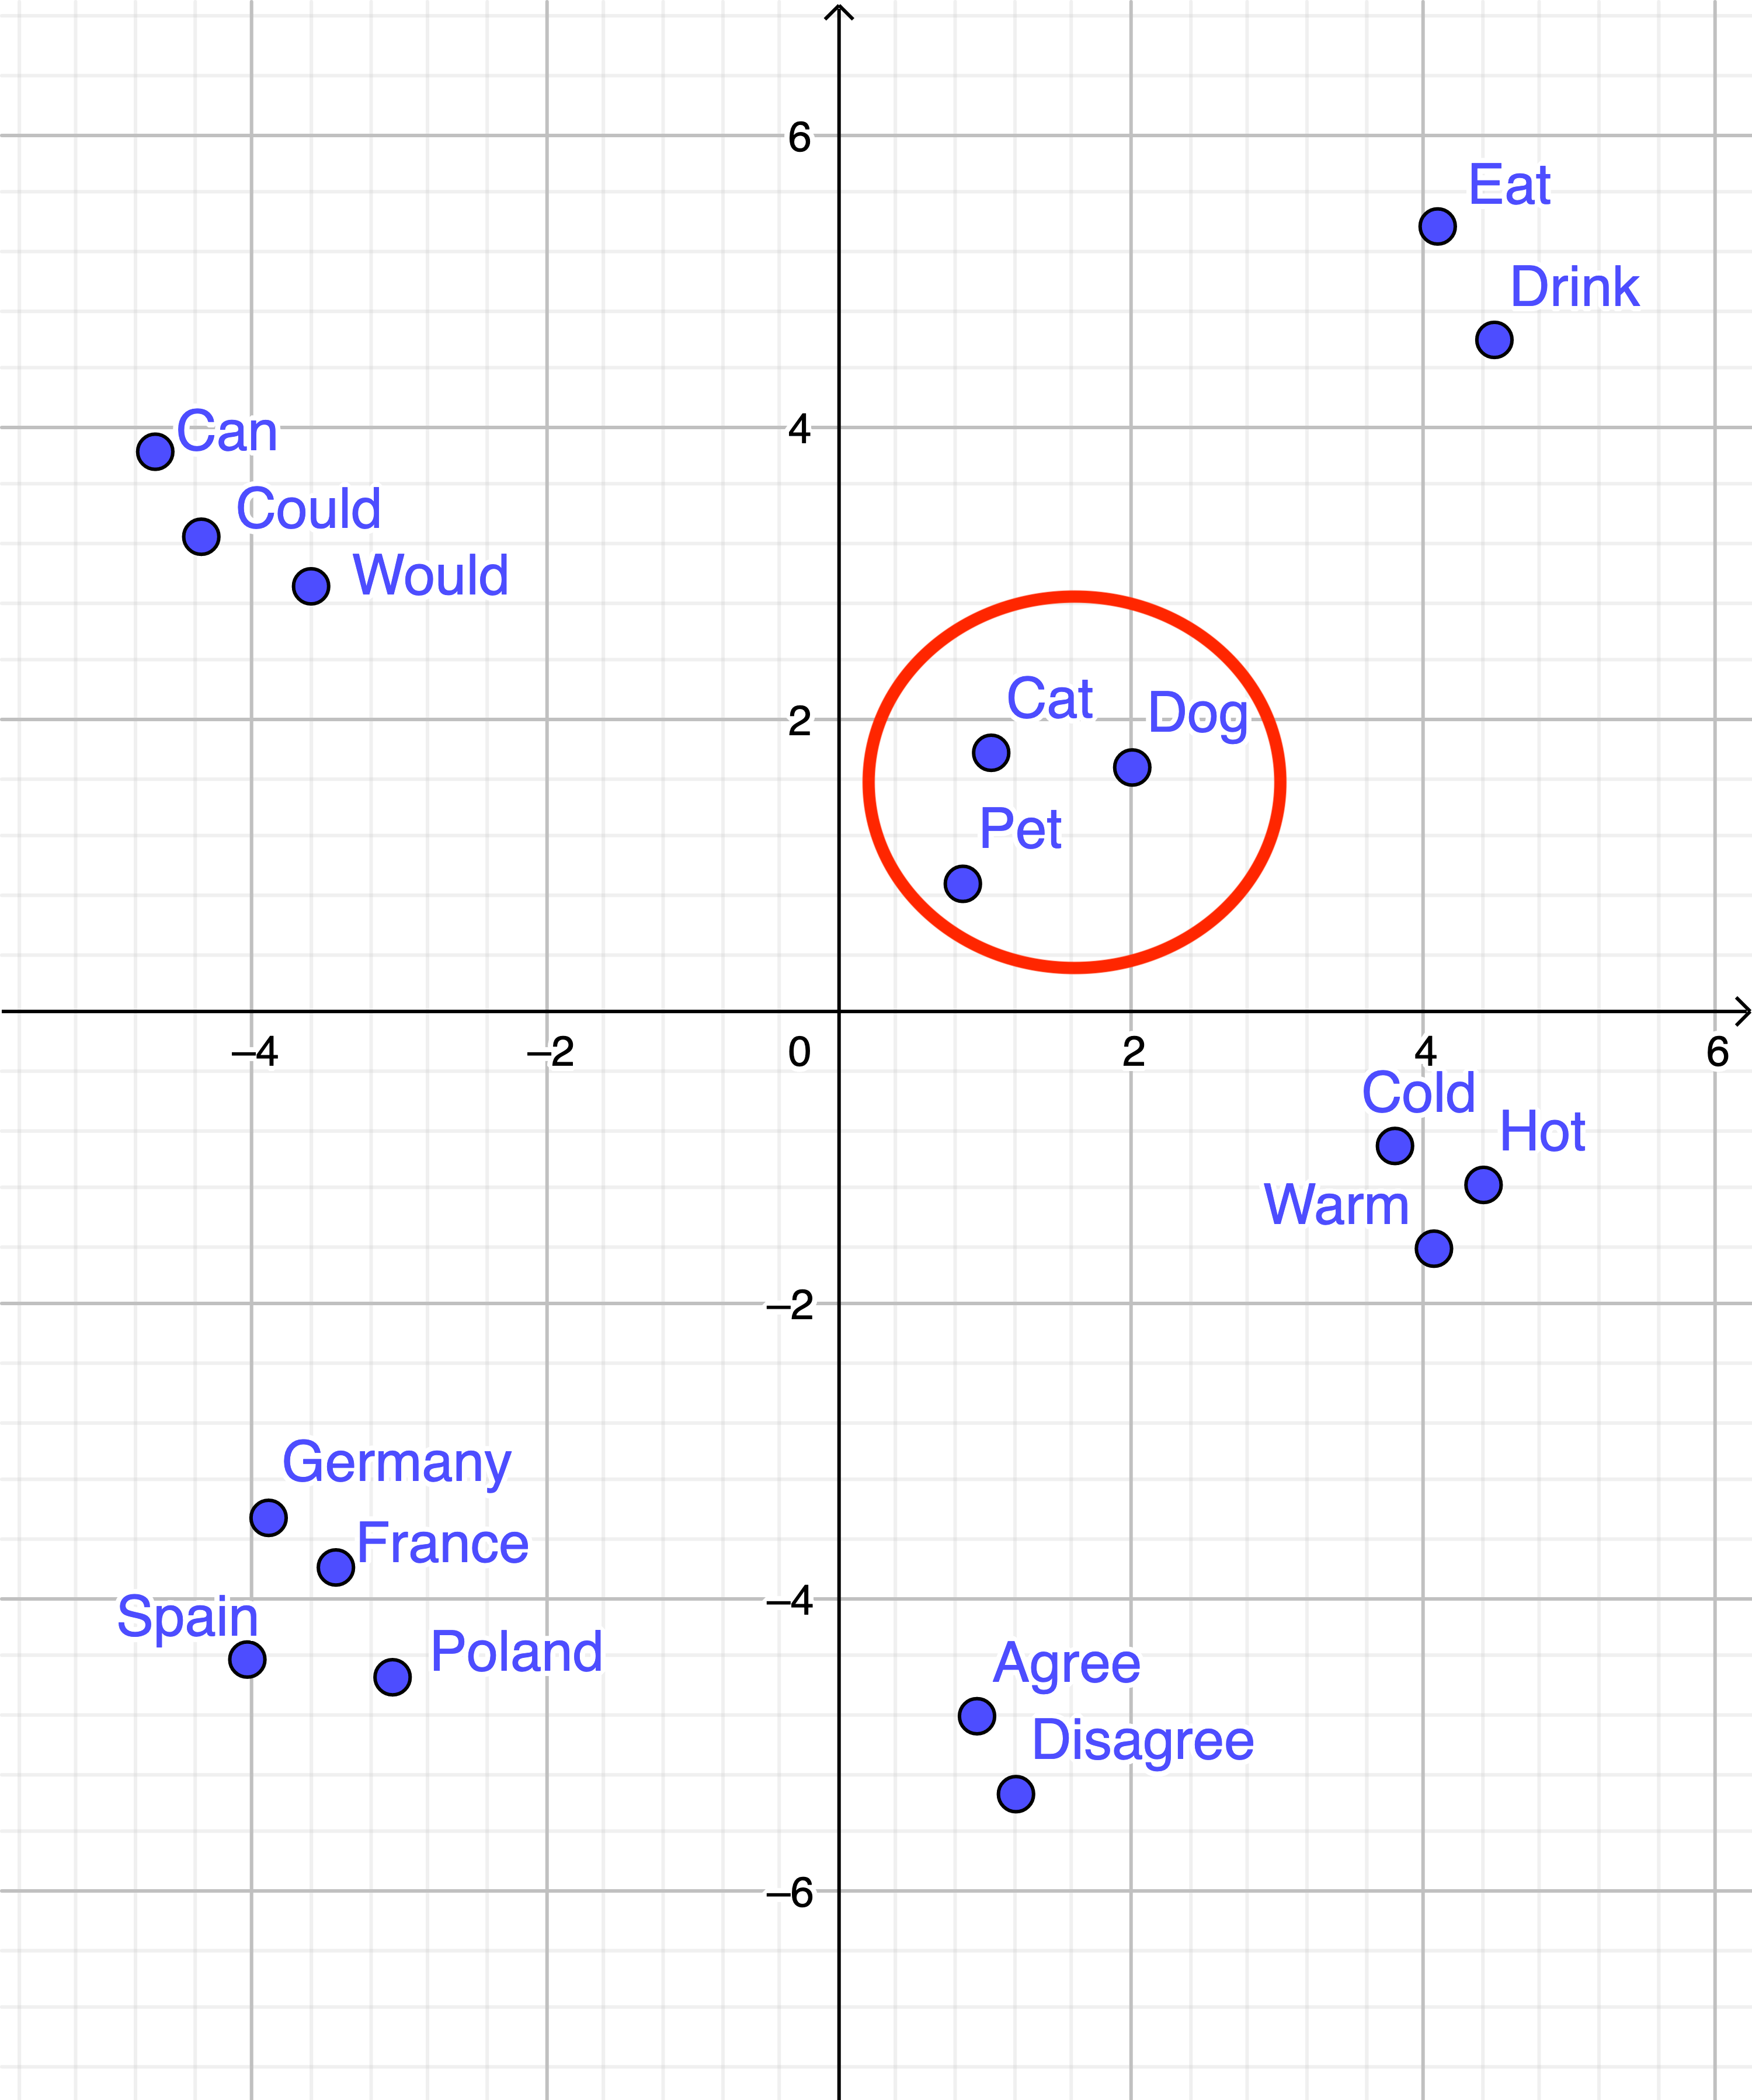
\includegraphics[width=4cm]{./figures/Group_hyponym}
	\end{figure}
		\begin{center}
		{Words are hyponym - hypernym}
		\end{center}
	\vspace{-0.5cm}

\end{frame}

\begin{frame}
	\frametitle{Word Embedding}

	\begin{figure}
		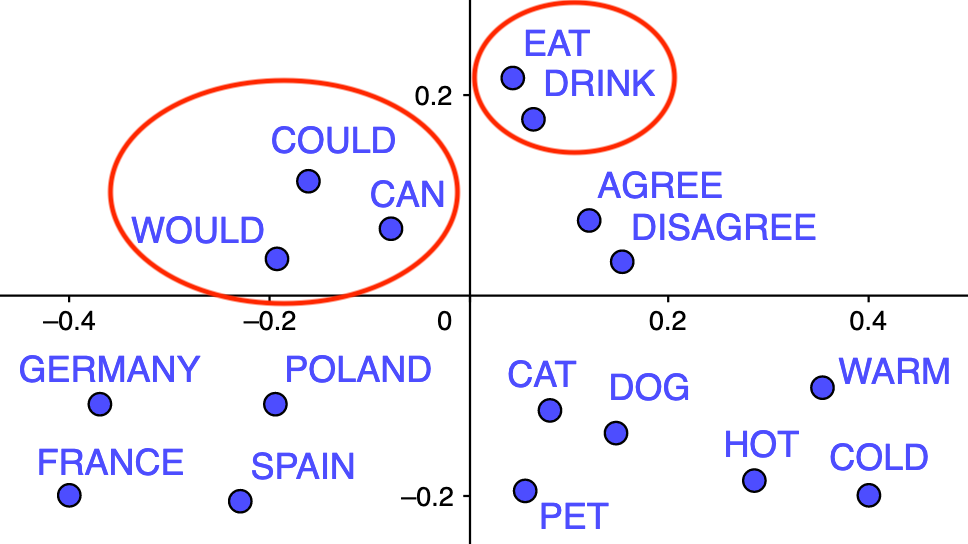
\includegraphics[width=4cm]{./figures/Group_context}
	\end{figure}
		\begin{center}
		{Words appear in similar context}
		\end{center}
	\vspace{-0.5cm}

\end{frame}


\begin{frame}
	\frametitle{How can we use it?}
	
	\begin{itemize}
		\item If user search for "Dell notebook battery size" we would like to match it also with "Dell laptop battery capacity"
		\item If user search for "Cracow Motel" we would like to match it also with "Krakow Hotel"
	\end{itemize}
	
\end{frame}











%%%%%%%%%%%%%%%%%%%%%%%%%%%%%%%%%%%%%%%%%%%%%%%%%%%%%%%%%%%%%%%%%%%%%%%%%%%%%%%%%%%%%%%%%%%%%%%%%%%
\begin{frame}
	\frametitle{Title of the Slide}
		\framesubtitle{Subtitle of the Slide: Use Only if Necessary\dots}
	
	\begin{itemize}
		\item Bulalet point 1.
		\item Bullet point 2 -e-- \alert{you can emphasise} a text.
	\end{itemize}

\end{frame}

%%%%%%%%%%%%%%%%%%%%%%%%%%%%%%%%%%%%%%%%%%%%%%%%%%%%%%%%%%%%%%%%%%%%%%%%%%%%%%%%%%%%%%%%%%%%%%%%%%%

\subsection{Subtopic 1} % Change, please!

%%%%%%%%%%%%%%%%%%%%%%%%%%%%%%%%%%%%%%%%%%%%%%%%%%%%%%%%%%%%%%%%%%%%%%%%%%%%%%%%%%%%%%%%%%%%%%%%%%%
\begin{frame}
	\frametitle{Title of the Slide}
		\framesubtitle{Slide without Bullets}

	Text:

	\vfill

	\begin{block}{}
		Blocks are good for important notions.
	\end{block}

	\vfill

	\begin{alertblock}{}
		Alertblocks are even better to catch the attention.
	\end{alertblock}

	\vfill

	\begin{alertblock}{Title}
		You can have the title in the (alert)block.
	\end{alertblock}

\end{frame}
%%%%%%%%%%%%%%%%%%%%%%%%%%%%%%%%%%%%%%%%%%%%%%%%%%%%%%%%%%%%%%%%%%%%%%%%%%%%%%%%%%%%%%%%%%%%%%%%%%%

\subsection{Subtopic 2} % Change, please!

%%%%%%%%%%%%%%%%%%%%%%%%%%%%%%%%%%%%%%%%%%%%%%%%%%%%%%%%%%%%%%%%%%%%%%%%%%%%%%%%%%%%%%%%%%%%%%%%%%%
\begin{frame}
	\frametitle{Title of the Slide}
		\framesubtitle{Slide with a Figure from a File}

	\begin{figure}
		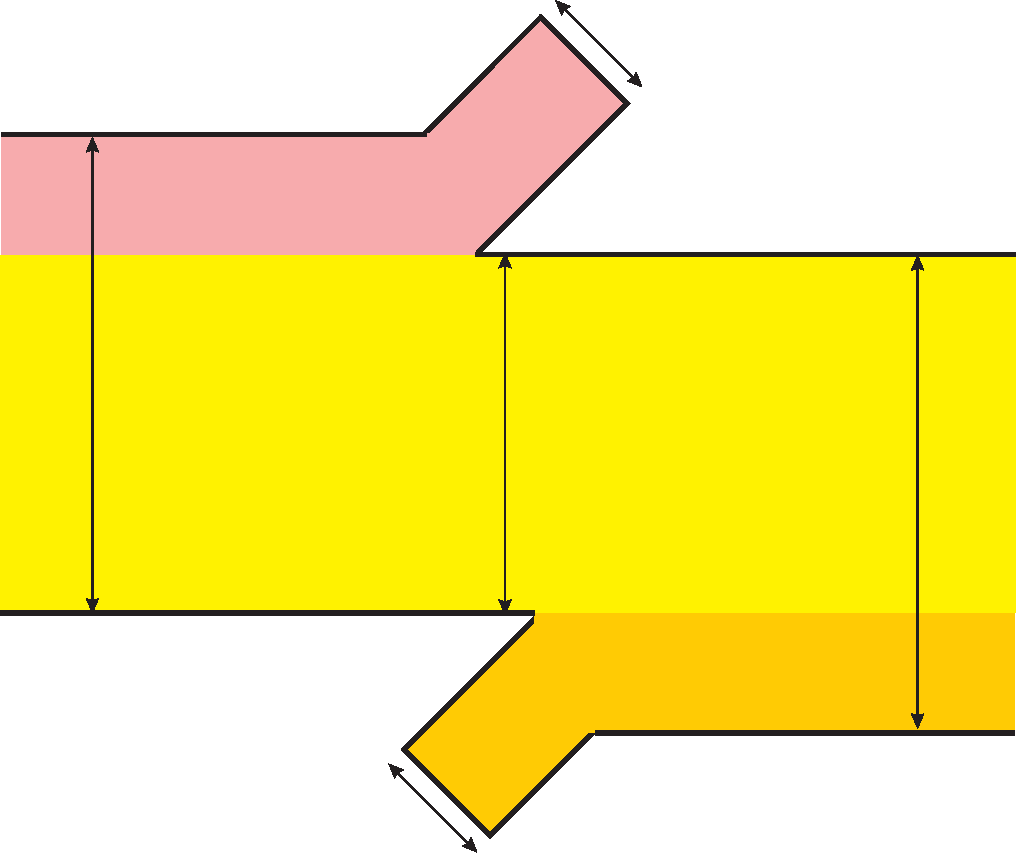
\includegraphics[width=6cm]{./figures/TIiK_channel_mutual_new}
		\caption{Caption of the figure}
	\end{figure}

	\vspace{-0.5cm}

	\tiny I am sorry that the example figures and the table concern the information theory \smiley

\end{frame}
%%%%%%%%%%%%%%%%%%%%%%%%%%%%%%%%%%%%%%%%%%%%%%%%%%%%%%%%%%%%%%%%%%%%%%%%%%%%%%%%%%%%%%%%%%%%%%%%%%%

%%%%%%%%%%%%%%%%%%%%%%%%%%%%%%%%%%%%%%%%%%%%%%%%%%%%%%%%%%%%%%%%%%%%%%%%%%%%%%%%%%%%%%%%%%%%%%%%%%%
\begin{frame}
	\frametitle{Title of the Slide}
		\framesubtitle{Slide with a Figure Drawn with \texttt{tikz}}

	\vspace{-0.5cm}

	\begin{changemargin}{-1cm}{-1cm}
		\begin{figure}
			\begin{tikzpicture}[x=2.5cm,y=2cm]
				\node[draw,thick,rectangle,fill=blue!25,align=center,text width = 1.5cm] (SOURCE) at (0,0) {\bfseries Source}; 
				\node[draw,thick,rectangle,fill=green!25,label=above:{\it Compression},align=center,text width = 1.5cm] (SOURCE_ENCODER) at (1,0) {\bfseries Source encoder}; 
				\node[draw,thick,rectangle,fill=magenta!25,label=above:{\it Security},align=center,text width = 2.00cm] (ENCRYPTION) at (2,0) {\bfseries Encryption}; 
				\node[draw,thick,rectangle,fill=red!25,align=center,text width = 1.5cm] (CHANNEL_ENCODER) at (3,0) {\bfseries Channel encoder};
				\node[align=center,text width = 1.5cm,yshift=1.05cm] at (CHANNEL_ENCODER) {\it Error\\protection}; 
				\node[draw,thick,rectangle,fill=gray!25,align=center,text width = 2.25cm] (MODULATOR) at (4,0) {\bfseries Modulator}; 
				\node[draw,thick,rectangle,fill=yellow!25,align=center,text width = 1.5cm] (CHANNEL) at (4,-1) {\bfseries Channel}; 
				\node[draw,thick,rectangle,fill=gray!25,align=center,text width = 2.25cm] (DEMODULATOR) at (4,-2) {\bfseries Demodulator}; 
				\node[draw,thick,rectangle,fill=red!25,align=center,text width = 1.5cm] (CHANNEL_DECODER) at (3,-2) {\bfseries Channel decoder}; 
				\node[draw,thick,rectangle,fill=magenta!25,align=center,text width = 2.00cm] (DECRYPTION) at (2,-2) {\bfseries Decryption}; 
				\node[draw,thick,rectangle,fill=green!25,align=center,text width = 1.5cm] (SOURCE_DECODER) at (1,-2) {\bfseries Source decoder}; 
				\node[draw,thick,rectangle,fill=blue!25,align=center,text width = 1.5cm] (SINK) at (0,-2) {\bfseries Sink}; 
				\node[starburst, fill=yellow, draw=red,line width=1pt,shift={(0.25,0.60cm)}] (NOISE) at (CHANNEL) {\color{red} \bf \tiny !};
	% 			\node[align=center,text width = 1.5cm] at (NOISE) {\color{red} Noise,\\errors,\\frauds};
				\draw[thick,->] (SOURCE) -- (SOURCE_ENCODER) ;
				\draw[thick,->] (SOURCE_ENCODER) -- (ENCRYPTION);
				\draw[thick,->] (ENCRYPTION) -- (CHANNEL_ENCODER);
				\draw[thick,->] (CHANNEL_ENCODER) -- (MODULATOR);
				\draw[thick,->] (MODULATOR) -- (CHANNEL);
				\draw[thick,->] (CHANNEL) -- (DEMODULATOR);
				\draw[thick,->] (DEMODULATOR) -- (CHANNEL_DECODER);
				\draw[thick,->] (CHANNEL_DECODER) -- (DECRYPTION);
				\draw[thick,->] (DECRYPTION) -- (SOURCE_DECODER);
				\draw[thick,->] (SOURCE_DECODER) -- (SINK);
				\coordinate (c1) at ($(CHANNEL_DECODER.south) + (0,-0.25cm)$);
				\draw[thick] (CHANNEL_DECODER) -- (c1);
				\draw[thick,->] (c1) -| (DEMODULATOR.south);
				\node at (3.5,-2.5) {\it Iterative decoding};
				\node[align=center,text width = 1.5cm] (SCT) at (1,-1) {Source\\coding\\theorem};
				\draw[->] (SCT) -- +(0,1.25cm);
				\draw[->] (SCT) -- +(0,-1.25cm);
				\node[align=center,text width = 1.5cm] (CCT) at (3,-1) {Channel\\coding\\theorem};
				\draw[->] (CCT) -- +(0,1.25cm);
				\draw[->] (CCT) -- +(0,-1.25cm);
				\draw[->] (CCT) -- +(0.5,0cm);
			\end{tikzpicture}
		\end{figure}		
	\end{changemargin}

	\vspace{-0.35cm}

	\tiny Source: \bibentry{Moon05a}.

\end{frame}
%%%%%%%%%%%%%%%%%%%%%%%%%%%%%%%%%%%%%%%%%%%%%%%%%%%%%%%%%%%%%%%%%%%%%%%%%%%%%%%%%%%%%%%%%%%%%%%%%%%

%%%%%%%%%%%%%%%%%%%%%%%%%%%%%%%%%%%%%%%%%%%%%%%%%%%%%%%%%%%%%%%%%%%%%%%%%%%%%%%%%%%%%%%%%%%%%%%%%%%
\begin{frame}
	\frametitle{Title of the Slide}
		\framesubtitle{Slide with a Table}
	
		\begin{table}
			\caption{Caption of the Table}
			\begin{center}
				\setlength\arrayrulewidth{2pt}
					\begin{tabular}{|>{\columncolor[rgb]{0,0.9,0.3}\color{white}}c|>{\columncolor[rgb]{0,0.9,0.1}\color{white}}c|}
					\hline
					\rowcolor[rgb]{0,0.5,0} \bfseries Data  & \bfseries Entropy \\
					\hline%
					\hline Plain text                        	  & $4{.}347$\\
					\hline Native executables	                   & $5{.}099$\\
					\hline Packed executables                   & $6{.}801$\\
					\hline Encrypted executables                & $7{.}175$\\
					\hline
				\end{tabular}
			\end{center}
		\end{table}

		\vfill

		\tiny Source: \bibentry{Lyda07a}.
\end{frame}
%%%%%%%%%%%%%%%%%%%%%%%%%%%%%%%%%%%%%%%%%%%%%%%%%%%%%%%%%%%%%%%%%%%%%%%%%%%%%%%%%%%%%%%%%%%%%%%%%%%

%%%%%%%%%%%%%%%%%%%%%%%%%%%%%%%%%%%%%%%%%%%%%%%%%%%%%%%%%%%%%%%%%%%%%%%%%%%%%%%%%%%%%%%%%%%%%%%%%%%
\begin{frame}
	
	\begin{center}
		\Huge \textbf{Thank you for your attention!}
	\end{center}

\end{frame}
%%%%%%%%%%%%%%%%%%%%%%%%%%%%%%%%%%%%%%%%%%%%%%%%%%%%%%%%%%%%%%%%%%%%%%%%%%%%%%%%%%%%%%%%%%%%%%%%%%%

%%%%%%%%%%%%%%%%%%%%%%%%%%%%%%%%%%%%%%%%%%%%%%%%%%%%%%%%%%%%%%%%%%%%%%%%%%%%%%%%%%%%%%%%%%%%%%%%%%%
\begin{frame}
	
	\begin{center}
		\Huge \textbf{Q \& A}
	\end{center}

\end{frame}
%%%%%%%%%%%%%%%%%%%%%%%%%%%%%%%%%%%%%%%%%%%%%%%%%%%%%%%%%%%%%%%%%%%%%%%%%%%%%%%%%%%%%%%%%%%%%%%%%%% % Change, please!

%%%%%%%%%%%%%%%%%%%%%%%%%%%%%%%%%%%%%%%%%%%%%%%%%%%%%%%%%%%%%%%%%%%%%%%%%%%%%%%%%%%%%%%%%%%%%%%%%%%
%%%%%%%%%%%%%%%%%%%%%%%%%%%%%%%%%%%%%%%%%%%%%%%%%%%%%%%%%%%%%%%%%%%%%%%%%%%%%%%%%%%%%%%%%%%%%%%%%%%
%%%%%%%%%%%%%%%%%%%%%%%%%%%%%%%%%%%%%%%%%%%%%%%%%%%%%%%%%%%%%%%%%%%%%%%%%%%%%%%%%%%%%%%%%%%%%%%%%%%
%%%%%%%%%%%%%%%%%%%%%%%%%%%%%%%%%%%%%%%%%%%%%%%%%%%%%%%%%%%%%%%%%%%%%%%%%%%%%%%%%%%%%%%%%%%%%%%%%%%
%%%%%%%%%%%%%%%%%%%%%%%%%%%%%%%%%%%%%%%%%%%%%%%%%%%%%%%%%%%%%%%%%%%%%%%%%%%%%%%%%%%%%%%%%%%%%%%%%%%
%%%%%%%%%%%%%%%%%%%%%%%%%%%%%%%%%%%%%%%%%%%%%%%%%%%%%%%%%%%%%%%%%%%%%%%%%%%%%%%%%%%%%%%%%%%%%%%%%%%

\bibliographystyle{plain}
\nobibliography{bibliographyfile} % your bibliography file

\end{document}